218. \begin{figure}[ht!]
\center{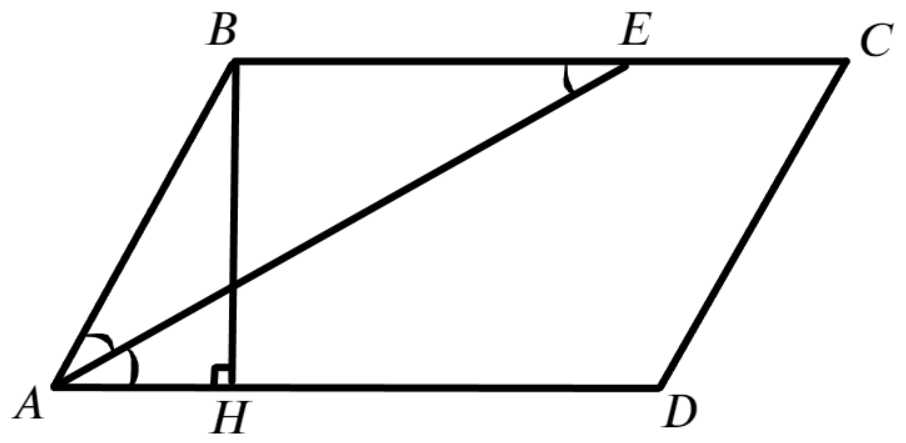
\includegraphics[scale=0.35]{g8-217.png}}
\end{figure}\\
Углы $EAD$ и $BEA$ равны как накрест лежащие, поэтому $\angle BAE=\angle EAD=\angle BEA$ и треугольник $BAE$ является равнобедренным, $AB=BE=1.$ Опустим высоту $BH,$ тогда $BH=AB\sin(60^\circ)=1\cdot\cfrac{\sqrt{3}}{2}=\cfrac{\sqrt{3}}{2}.$ Площадь параллелограмма $ABCD$ равна $S=BH\cdot AD=\cfrac{\sqrt{3}}{2}\cdot(1+3)=2\sqrt{3}.$\\
